\subsection{Site Internet}

    \subsubsection{Seconde soutenance}

    \textbf{réalisation}

    La réalisation d'un site internet pour le projet était un objectif
    programmé pour la deuxième soutenance, ce qui est maintenant chose faite.
    Pour ce dernier, nous avons retenu Bootstrap, qui est une collection
    d'outils HTML, CSS et Javascript apportant des éléments de site
    esthétiques et simples à utiliser. Le thème Freelancer, élégant et sobre,
    nous a tapé dans l'oeil ; cependant, comme c'est un thème très 
    communément utilisé, nous changerons à terme certains éléments afin 
    d'y apposer notre signature. Bootstrap Studio nous a aidés à réaliser
    un site dynamique, mais ne s'est pas montré à la hauteur de nos espérances
    en matière de personnalisation. En effet, on ne peut pas modifier
    le code HTML (seulement ajouter / supprimer des blocs ou éditer les
    attributs), et les styles CSS ne sont modifiables qu'en créant une copie
    du fichier CSS d'origine.

    \begin{figure}[hbt!]
        \centering
        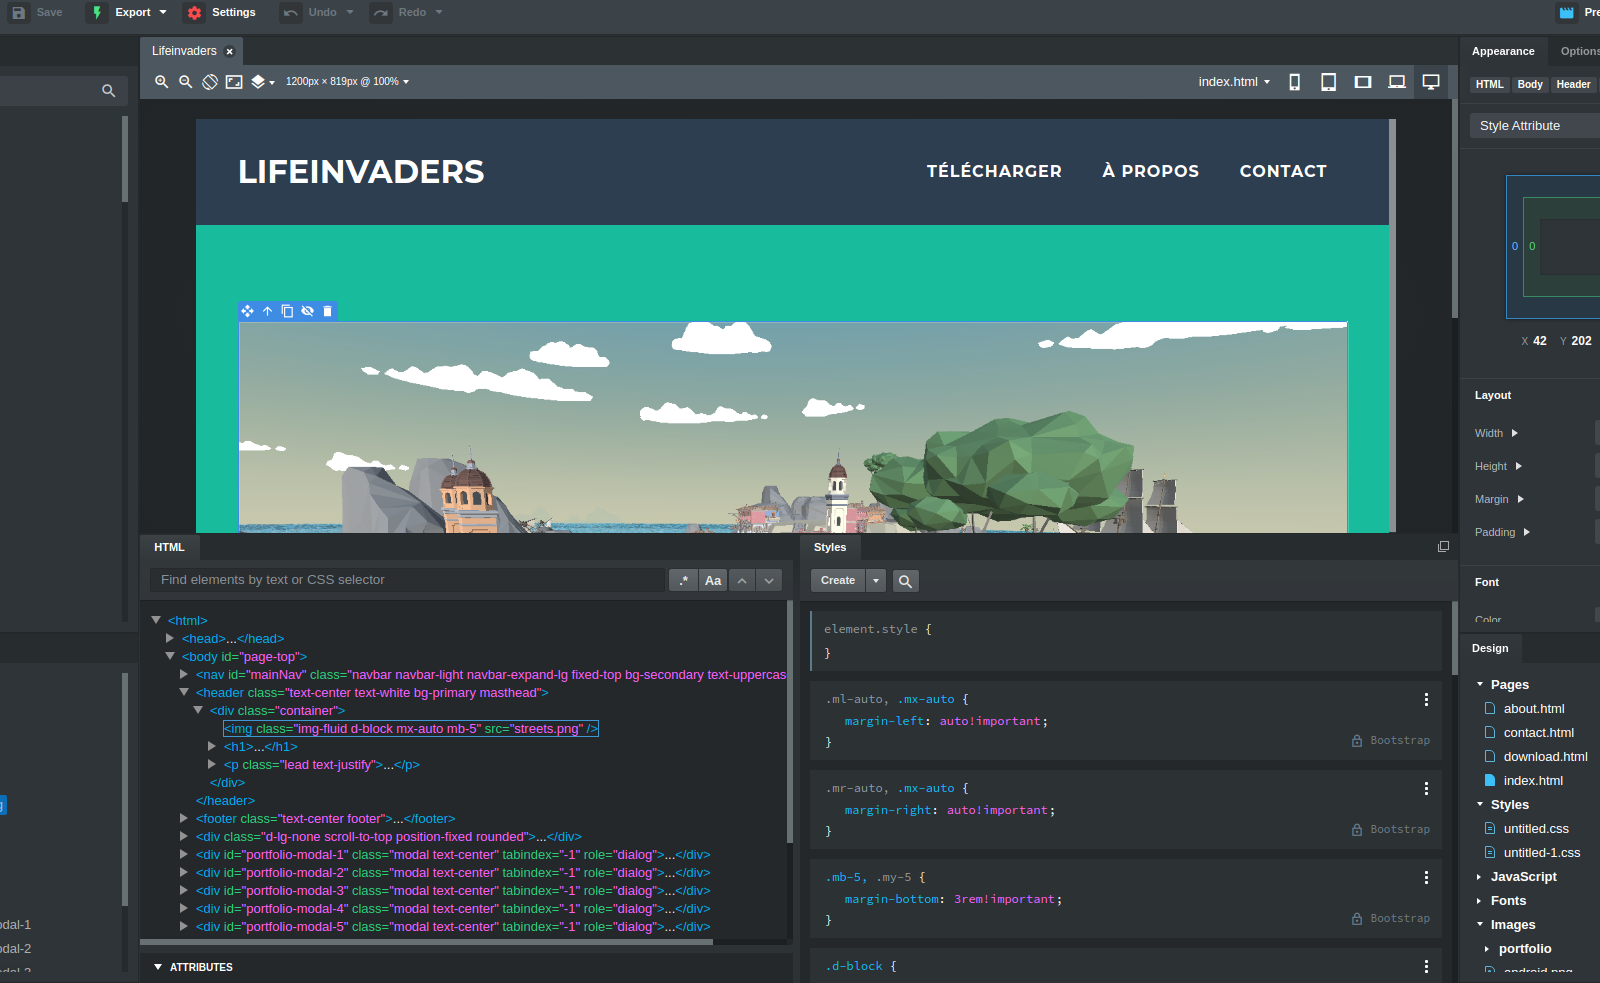
\includegraphics[scale=0.37]{bootstrap_studio.png}
        \caption{Le logiciel Bootstrap Studio}
    \end{figure}

    La conception du site s'est donc déroulée en deux parties. En premier, la création
    d'une base grâce à BootStrap Studio, en modifiant les images, textes et titres présents, ainsi
    que d'autres chose un peu plus minutieuses, comme la modification de tableaux et des encarts personnalisés.
    Ensuite, la modification plus poussée des options verouillées par BootStrap Studio, comme l'ajout de liens 
    sur les images, ou encore la modification des titres et favicons.

    \begin{figure}[hbt!]
        \centering
        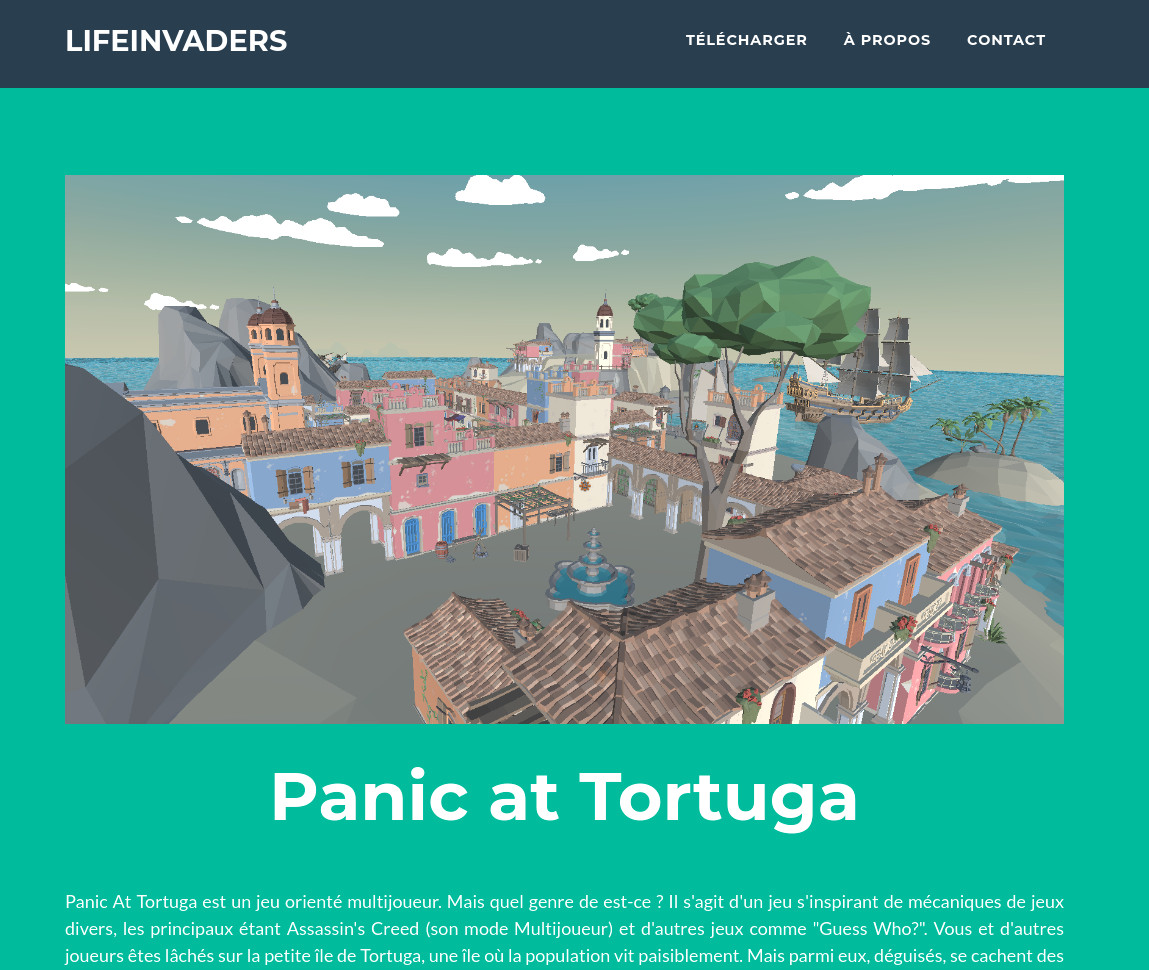
\includegraphics[scale=0.376]{website.png}
        \caption{Aperçu de notre site}
    \end{figure}


    \textbf{Hébergement}

    L'hebergement de petits sites comme celui-ci n'étant pas très contraignant,
    nous avons décidé d'utiliser un hébergeur gratuit, car ces derniers
    sont généralement largement suffisants. Après avoir cherché parmi les
    solutions proposées, nous avons décidé d'utiliser la solution 
    \textit{Github Pages}, qui permettait d'avoir une extension "sérieuse"
    (nous préférons une site qui finit par github.io que par wix.com),
    ainsi qu'une gestion de ce dernier très simplifiée, grâce au gestionnaire de versions.
    Ainsi, tout comme pour le projet, les versions sont gérées en trois commandes 
    (git add, git commit , git push), et la limite de taille de 1 Go est plus que suffisante pour quatre pages html. 


    \begin{figure}[hbt!]
        \centering
        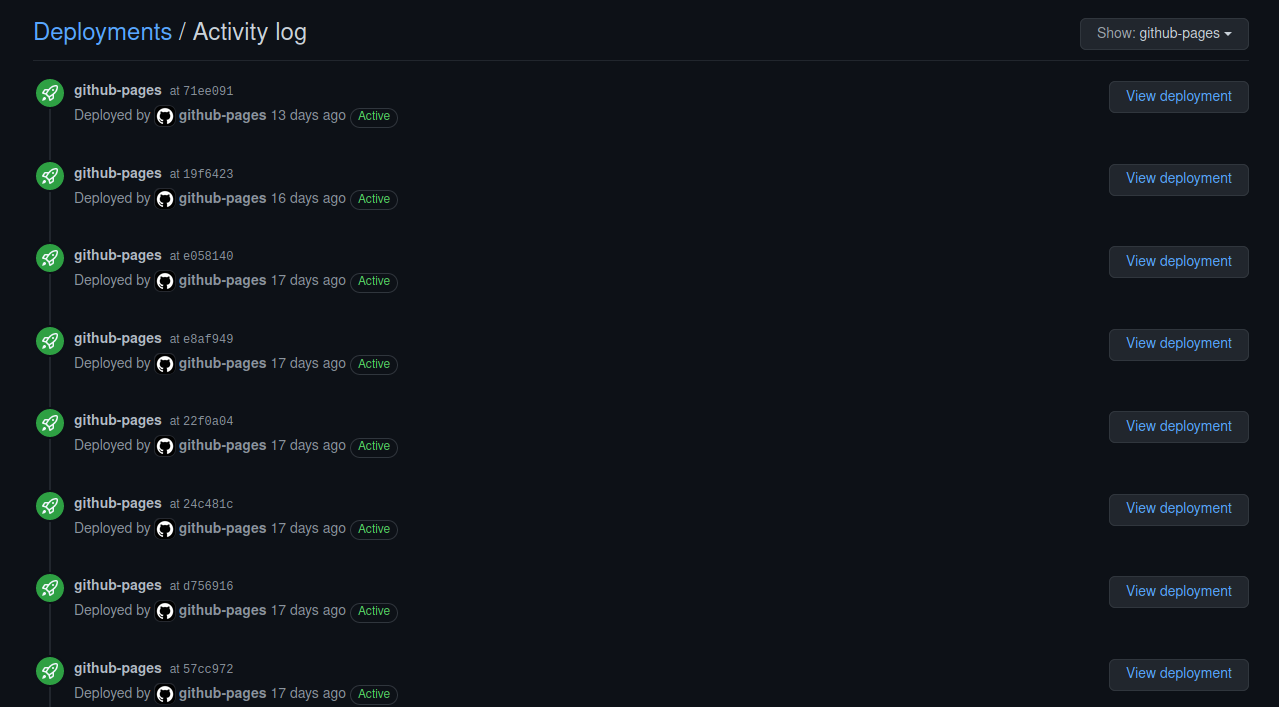
\includegraphics[scale=0.47]{deployment_versions.png}
        \caption{Liste des différentes versions du site}
    \end{figure}

    
    \textbf{Améliorations futures}

    La création et la maintenance d'un page recensant les nouveautés apportées par chaque version est un des 
    principaux points prévus pour la dernière soutenance, afin de pouvoir voir l'évolution du projet au fil des 
    mois et d'être informé des dernières mises à jour du jeu. Un autre aspect important à développer est l'indentité
    visuelle du site, afin de le rendre unique. Pour cela,  nous comptons utiliser de polices de caractères originales 
    et de couleurs vives et attrayantes. Des éléments dynamiques seront également nécéssaires à rendre le site agréable 
    à consulter.